\chapter{Implementacja} 
\label{sec:implementation}
W tym rozdziale opisane są szczegóły techniczne zastosowanych rozwiązań.

\section{Istniejące implementacje}
	Istnieją także inne modele jeżdżących robotów na kołach szwedzkich.
	Można z nich brać przykład i sugerować się źródłami kodu i budową modeli.

	Kuka Youbot jest popularnym robotem wielokierunkowym. Jego modele są domyślnie dostępne w różnych symulatorach, między innymi w Gazebo i V-Repie, które są dobrymi kandydatami do 
	użycia w projekcie. Tylko w przypadku V-Repa, istnieje wstępny sterownik do którego da się wysyłać odpowiednie wartości zadanej prędkości liniowej i kątowej, a on nadaje odpowiednie prędkości kołom, aby odpowiednio poruszać modelem.
	Wersja dla Gazebo jest statycznym obiektem z błędnie ustanowionymi przegubami, jego efektory nie są zaimplementowane.
	
	Dodatkowo, V-Rep posiada wbudowane dwa inne pojazdy o napędach kół Mecanum i czujnikach laserowych.
	Zewnętrzne modele także pomogą przy wstępnej weryfikacji zachowania się budowanego tutaj modelu, czy nie zachowuje się nadzwyczaj dziwnie w pierwszych fazach projektu.

	Ze względu na niezwykle zaawansowany obiekt kół i kształt rolek, ważne jest aby uprościć model, poprzez zamianę niektórych składowych i dodanie sztucznych więzów.
	Całościowy model może być zbyt skomplikowany, aby maszyny symulacji mogły go obliczać w czasie rzeczywistym.
	Dokładny model także jest znacznie trudniej poprawnie wymodelować, ze względu na liczne tarcia i poślizgi rolek.
	Proponowane uproszczenia modeli opisane są w sekcji \ref{sec:omnivelma}.
	
\section{Model 3D}
	Model 3D bazy mobilnej, opisany równaniami matematycznymi, powinien mieć zachowanie zbliżone do oryginału, najbardziej jak to tylko możliwe.
	Musi uwzględniać masy i momenty bezwładności elementów składowych, a także wszystkie tarcia.
	Model obejmuje więzy na ruchome elementy, takie jak koła i rolki, aby umożliwić symulację przegubów.

	Model składa się z elementów, odwzorowujących rzeczywiste części składowe bazy mobilnej.
	Elementy posiadają takie cechy, jak:
	\begin{itemize}
		\item Pozycja w modelu.
		\item Masa.
		\item Moment bezwładności.
		\item Kształt fizyczny.
		\item Materiał fizyczny.
		\item Wygląd.
	\end{itemize}

	Dodatkowo, należy uwzględnić wszystkie więzy, w postaci symulowanych przegubów.
	W przypadku tej bazy istnieje typ więzów o jednym stopniu swobody, używany przy połączeniu przedniej i tylnej części platformy, oraz 
	jako piasty kół i rolek. Można także uznać, że więzy bez stopni swobody używane są do trwałego połączenia czujników z platformą i transportowanym robotem.
	Więzy mogą oddziaływać siłą na elementy do których są podłączone, symulując silniki.

	Elementy składowe i symulowane przeguby oddziałują bezpośrednio z maszyną do symulacji fizycznej. 
	To kształt, masy i momenty bezwładności brył są argumentami funkcji liczących.
	Maszyna symulacyjna oblicza odpowiednie prędkości i nadaje je podanym obiektom w podobny sposób, jak ma to miejsce w rzeczywistości.

	Do modelu doczepia się wirtualne czujniki, generujące odpowiednie dane na podstawie symulacji i rozkładu losowego.
	Nie są to pełne dane o stanie modelu, jakie posiada maszyna do symulacji, gdyż czujniki fizyczne również nigdy nie mają pełnej informacji o stanie urządzenia.
	Należy dodać losowy szum i błędy, aby przybliżyć ich zachowanie do rzeczywistych czujników.

	Dla odpowiedniej wizualizacji symulacji, można wykorzystać istniejący model CAD do stworzenia siatki trójwymiarowej i nadania symulowanemu obiektowi wyglądu zbliżonego do fizycznego robota. Nie ma to znaczenia dla przebiegu symulacji, gdyż ta część nie bierze udziału w obliczeniach maszyny symulującej fizykę.

	W środowisku wirtualnym należy stworzyć program o podobnym działaniu.
	Powinien przyjmować dane w dokładnie takim samym formacie, jak opisany wyżej układ, aby był łatwo wymienialny na sterownik fizycznego urządzenia bez ingerencji w główny program sterujący.
	Zamiast zamieniać odczytane dane na analogowe wartości, sterownik wywołuje odpowiednie funkcje maszyny symulacyjnej, aby wywołać taki sam efekt, co na rzeczywistym efektorze, lecz w wirtualnej przestrzeni symulacji.
	Jako argumenty podaje parametry fizyczne symulowanego obiektu, oraz przyłożone siły.

	
\section{Ogólne typy pakietów}
	Pakiety można podzielić na kilka typów, w zależności od sposobu implementacji.
	Wszystkie programy napisane są w języku C++ i korzystają z nowoczesnych rozwiązań języka jak referencje i sprytne wskaźniki.
	
	\subsection{Program wykonywalny w ROS}
		\label{sec:ros_exe}
		Jest to prosty program, który korzysta z kilku funkcji ROSa, między innymi:
		\begin{itemize}
			\item Inicjalizacja węzła.
			\item Stworzenie nadajnika strumienia wiadomości.
			\item Stworzenie odbiornika strumienia wiadomości.
			\item Zawieszenie procesu.
			\item Generowanie logów, jak informacje i ostrzeżenia.
		\end{itemize}
		
		\subsubsection{Inicjalizacja}
			Na początku głównej funkcji programu \mintinline{cpp}{int main(int argc, char** argv)}, należy podać argumenty wywołania programu
			do funkcji inicjalizującej ROSa. Ta funkcja odczytuje argumenty dotyczące tej programowalnej struktury ramowej i modyfikuje zmienne w razie problemów, usuwając niektóre argumenty, aby reszta programu parsowała poprawne dane.
			\begin{minted}{cpp}
void ros::init (int& argc, 
	char** argv, 
	const std::string& name, 
	uint32_t options = 0)
			\end{minted}
			Ta funkcja przyjmuje także nazwę nowego węzła, jaka zostanie zgłoszona do demona ROS oraz flagi opisujące inicjalizację.
			Nazwa musi być unikalna dla całego systemu, nie mogą działać dwa węzły o tej samej nazwie.
			Flagi opisują, czy program powinien mieć zawieszone wypisywanie logów, czy nazwa powinna być anonimowa (co pozwala na uruchomienie wielu instancji tego samego programu)
			oraz czy program powinien się zakończyć na otrzymanie sygnału systemowego \texttt{SIGINT}.
			
			Następnie program parsuje argumenty wywołania, w zależności od tego, jakie zadanie ma wykonywać.
			
		\subsubsection{Stworzenie nadajnika}
			Kolejnym krokiem jest otwarcie komunikacji poprzez strumienie wiadomości z innymi węzłami.
			W tym celu tworzy się obiekt węzła, obiekt klasy \mintinline{cpp}{ros::NodeHandle}, którego konstruktor nie przyjmuje argumentów.
			Ten obiekt służy do komunikacji ze środowiskiem ROSa, pozwala na tworzenie nadajników i odbiorników.
			Programista musi jedynie się upewnić, aby zachować referencję do obiektu przez cały czas życia programu, gdyż destrukcja obiektu odłącza 
			program od demona ROSa.
			\begin{minted}{cpp}
template<class M>
Publisher ros::NodeHandle::advertise (const std::string& topic,
	uint32_t queue_size,
	bool latch = false)	
			\end{minted}
			Korzystając z obiektu węzła, można zarejestrować, za pomocą powyższej funkcji, nowe nadajniki strumienia wiadomości.
			Jest to metoda szablonowa, to oznacza, że przy wywołaniu należy podać typ wiadomości, jaką węzeł powinien nadawać.
			Następne argumenty to nazwa strumienia, wielkość bufora wysłanych wiadomości, oraz opcjonalny argument, decydujący o tym czy ostatnia nadana wiadomość powinna
			być buforowana i wysłana natychmiast na podłączenie się nowego odbiorcy do tego strumienia. Metoda zwraca obiekt nadajnika który to może być użyty do nadawania wiadomości.
			\begin{minted}{cpp}
template<class M>
void ros::Publisher::publish(const M& message) const
			\end{minted}		
			Za pomocą operatora negacji można sprawdzić, czy stworzenie obiektu przebiegło pomyślnie, a jeśli nie, poinformować użytkownika i zakończyć program.
			
			Wysłanie wiadomości to stworzenie nowego obiektu klasy wiadomości i podanie go do metody obiektu nadajnika.
			To także jest funkcja szablonowa, korzystająca z typu podanego przy tworzeniu obiektu.
			
		\subsubsection{Stworzenie odbiornika}
			W nieco inny sposób należy stworzyć odbiornik strumienia wiadomości.
			Po każdej odebranej wiadomości, wywoływana jest podana w argumencie funkcja, która przyjmuje i parsuje wiadomość.
			Można to porównać do działania przerwań systemowych.
			\begin{minted}{cpp}
template<class M>
Subscriber ros::NodeHandle::subscribe(const std::string& topic,
	uint32_t queue_size,
	void(*)(M) handler,
	const TransportHints& transport_hints = TransportHints())
			\end{minted}
			Podana metoda, podobnie, jak w nadajniku, jest metodą obiektu węzła.
			Przyjmuje nazwę strumienia wiadomości, wielkość bufora, wskaźnik na funkcję obsługi oraz opcjonalnie informacje dotyczące połączenia.
			Te informacje to takie jak typ używanego protokołu (datagramowy, czy połączeniowy), wielkość pakietu sieciowego, itp.
			
			Metoda posiada wiele różnych odmian, w zależności od sposobu podania funkcji obsługującej. Zamiast funkcji, może być to na przykład funktor.
			Wywołanie tworzy nowy obiekt odbiornika, na którym przy normalnym działaniu nie trzeba wywoływać żadnych metod.
			Jednakże, nadal należy posiadać referencję do niego, gdyż destrukcja obiektu automatycznie zamyka połączenie.
			
			Jeśli strumień wiadomości o takiej nazwie nie istnieje, metoda nie zwraca błędu. To ponieważ nadal może w przyszłości pojawić się
			nadajnik o odpowiedniej nazwie. Dodatkowo to utrudniałoby jednoczesne uruchamianie kilku węzłów zależnych od siebie, gdyż należałoby się upewnić, że
			nadajniki uruchomią się pierwsze. A także nie pozwalałoby na połączenie strumieni wiadomości w cykle.
			
		\subsubsection{Wypisywanie logów}
			Pomimo, że program może zwracać dane na standardowe wyjście i błąd, użycie funkcji ROSa pozwala na selektywne ustawienie minimalnej ważności zwracanych powiadomień.
			ROS także koloruje tekst i dodaje przedrostek z czasem nadania powiadomienia.
			
			\begin{figure}[h]
			\begin{minted}{cpp}
ROS_INFO(...)
ROS_INFO_STREAM(...)
			\end{minted}
			\caption{Makra ROSa, wypisujące powiadomienia.}
			\label{code:ros_logging}
			\end{figure}
			
			Używa się makr z rysunku \ref{code:ros_logging}, wszystkie makra są podane w dwóch typach, pierwsze pozwala na użycie argumentów
			w sposób charakterystyczny dla systemowej funkcji \texttt{printf}, a drugie przez strumienie języka C++.
			
			Tekst \texttt{INFO} może być zastąpiony przez jeden z pięciu priorytetów powiadomienia: \texttt{DEBUG}, \texttt{INFO}, \texttt{WARN}, \texttt{ERROR} i \texttt{FATAL}.
			
		\subsubsection{Zawieszenie procesu}
			Wywołanie \mintinline{cpp}{ros::spin()} powoduje zawieszenie się głównego wątku programu. 
			W ten sposób program będzie działał jedynie na odbiór wiadomości.
			Istnieją funkcje systemowe, które pozwalają na dokonanie tego samego, lecz API ROSa jest prostsze w użyciu, a także może wykonywać dodatkowe akcje
			związane z demonem.
			
		\subsubsection{Przykład}
			Przykładowe użycie powyższych metod przy implementacji prostego filtra wiadomości. 
			Ten kod tworzy nadajnik i odbiornik wiadomości, zawierającej prędkość liniową i kątową, a następnie na odbiór każdej wiadomości,
			przekazuje dalej jedynie prędkość liniową w płaszczyźnie platformy i prędkość kątową wokół osi Z, skierowanej w górę.
			Dzięki temu robot nie otrzyma sterowania w niemożliwym do poruszania się kierunku.
			
			Następnie wątek główny zostaje uśpiony, gdyż program działa jedynie w systemie akcja-reakcja.
			Wysyła wiadomość jedynie po otrzymaniu innej.
			
			\begin{minted}{cpp}
#include <iostream>
#include <string>
#include <ros/ros.h>
//nagłówek dla funkcji wypisujących powiadomienia
#include <ros/console.h>
//nagłówek z klasą wiadomości
#include <geometry_msgs/Twist.h>
			
//obiekt nadajnika
ros::Publisher publisher;
			
//funkcja obsługi odbioru wiadomości
void callbackFun(const geometry_msgs::Twist::ConstPtr& msg)
{
	//nowy obiekt typu wiadomość 
	//konstruktor zeruje wszystkie pola
	geometry_msgs::Twist newTwist;
	newTwist.linear.x = msg->linear.x;
	newTwist.linear.y = msg->linear.y;
	newTwist.angular.z = msg->angular.z;
	//wysyłanie wiadomości
	publisher.publish(newTwist);
}

int main(int argc, char** argv)
{
	//inicjalizacja
	ros::init(argc, argv, "filtrownica");

	//nazwa strumienia wejściowego
	std::string inTopic;
	//nazwa strumienia wyjściowego
	std::string outTopic;
	
	//...parsowanie argumentów argc i argv 
	//w celu odczytania powyższych zmiennych

	//obiekt węzła
	ros::NodeHandle handle;
	
	//stworzenie nadajnika wiadomości
	publisher = handle.advertise<geometry_msgs::Twist>(outTopic, 1000);
	if(!publisher)
	{
		ROS_FATAL_STREAM("Nie udało się stworzyć nadajnika " << outTopic);
		return -1;
	}
	
	//stworzenie odbiornika wiadomości
	ros::Subscriber subscriber;
	subscriber = handle.subscribe<geometry_msgs::Twist>(inTopic, 
		1000, callbackFun);
	if(!subscriber)
	{
		ROS_FATAL_STREAM("Nie udało się stworzyć odbiornika " << inTopic);
		return -1;
	}

	//zawieszenie wykonywania głównego wątku
	ros::spin();
	return 0;
}
			\end{minted}
			
	\subsection{Wtyczka Gazebo}
		\label{sec:gazebo_bib}
		Wtyczka do symulatora Gazebo jest klasą, dziedziczącą po klasie \texttt{ModelPlugin}, lub
		w przypadku modelu czujnika po \texttt{SensorPlugin}.
		Jest kompilowana do postaci biblioteki i ładowana dynamicznie przy uruchomieniu symulatora.
		Gazebo, prócz wywołania ewentualnego konstruktora, wywołuje metodę wirtualną
		\begin{minted}{cpp}
void Load(physics::ModelPtr parent, sdf::ElementPtr sdf)
		\end{minted}
		która to posiada argument typu sprytny wskaźnik na obiekt modelu, który obsługuje ta wtyczka, oraz wskaźnik na element pliku SDF, opisujący go.
		
		Jeśli chodzi o komunikację z ROSem, to może ona być zrealizowana identycznie, jak w sekcji \ref{sec:ros_exe}, 
		z tą różnicą, że nie jest wymagana inicjalizacja, gdyż logicznie cały symulator działa jak jeden węzeł.
		Również, jeśli chodzi o referencje do obiektów, to należy je zachować po opuszczeniu metody \texttt{Load}, to znaczy
		że obiekty węzła, nadawców i odbiorców powinny być przechowywane jako pola stworzonej klasy.

		\subsubsection{Wywołanie na kroki symulacji}
			Główną mechaniką używaną u wtyczek jest periodyczne wywołanie kodu co każdy krok symulacji.
			Pozwala to na przykład nadawać aktualną pozycję modelu.
			Gazebo obsługuje kilka zdarzeń, wywoływanych na różne części symulacji.
			Ten, do którego należy się podłączyć to \texttt{WorldUpdateBegin}, połączenie się do tego zdarzenia wywołuje następującą metodę:
			\begin{minted}{cpp}
ConnectionPtr Connect(const boost::function< T > & _subscriber)	
			\end{minted}
			Oznacza to tyle, że do podłączenia można użyć funktorów z biblioteki \texttt{boost}, lub lepiej, ze standardu C++.
			Przykładowe podłączenie do własnej zdefiniowanej metody \texttt{OnUpdate} może wyglądać w ten sposób:
			\begin{minted}{cpp}
event::ConnectionPtr connection = event::Events::ConnectWorldUpdateBegin(
	std::bind(&MyModelDriver::OnUpdate, this));
			\end{minted}
			Należy zatrzymać zwrócony sprytny wskaźnik do połączenia.
			
\section{Mechanika macierzy przekształceń jednorodnych}
	\label{sec:frames}
	Komunikacja poprzez pakiety wiadomości nie jest jedynym sposobem na przekazywanie informacji w środowisku ROS.
	Istnieje także mechanika macierzy transformacji \texttt{TF2}.
	Jest to idea podobna do niezaimplementowanej funkcjonalności Gazebo, ale nie jest automatyczna i nie ogranicza się tylko do jednego programu.
	
	Macierz transformacji jest informacją o aktualnym położeniu i orientacji jakiegoś obiektu względem innego.
	Polega na wysłaniu pakietu typu \texttt{geometry\_msgs/TransformStamped} prosto do demona ROS.
	Pakiet zawiera:
	\begin{itemize}
		\item Nagłówek z czasem nadania wiadomości i identyfikatorem, oraz informacją względem jakiej pozycji podane są poniższe dane.
		\item Nazwa nowej pozycji, jaka powstanie po zastosowaniu podanej transformacji do określonej w nagłówku pozycji.
		\item Lokalne położenie.
		\item Lokalna orientacja.
	\end{itemize}
	Demon ROSa następnie zbiera wszystkie dane ze wszystkich nadających węzłów i oblicza hierarchę przekształceń obiektów.
	Zwraca te dane na zapytania od innych węzłów.
	
	Przykładowo, gdyby symulacja robota nie odbywałaby się w przestrzeni wirtualnej, w maszynie symulacyjnej fizyki, 
	informacja o dokładnym położeniu obiektu składowego w lokalnym układzie współrzędnych wcale nie musiałaby być łatwo dostępna.
	Ma to szczególne znaczenie dla skomplikowanych mechanizmów, na przykład wielosegmentowego ramienia manipulacyjnego.
	Obliczenie położenia i orientacji końcówki ramienia wymagałoby informacji o aktualnych pozycjach wszystkich poniższych segmentów.
	Która część systemu miałaby zajmować się obliczeniami i gdzie przekazywać te informacje?
	
	Demon ROSa działa tutaj jak trzecia strona, zbierająca dane od sterowników i obliczająca położenia i orientacje wszystkich punktów.
	W takim przypadku, każdy segment symulacji mógłby przekazywać swój identyfikator, identyfikator obiektu którym steruje i jego pozycję do demona ROSa.
	Inne programy, na przykład do wizualizacji, mogłyby wtedy zapytać się demona o dokładne pozycje przegubów w przestrzeni kartezjańskiej, a on obliczyłby je i zwrócił wynik.
	
	W symulacji platformy wielokierunkowej, mechanika przekształceń jednorodnych jest potrzebna, gdyż wiadomość zwierająca pomiary z czujnika laserowego nie posiada informacji o aktualnej pozycji samego czujnika w przestrzeni, a jedynie wspomniany identyfikator. 
	Orientacja i położenie potrzebne są programowi obliczającemu pozycję z czujników i ewentualnemu wizualizatorowi samych danych.
	
	
	\begin{table}
		\centering
		\begin{tabular}{l r}
			Punkt względny & Identyfikator \\
			\hline
			Stały środek mapy & \texttt{map} \\
			Środek platformy & \texttt{omnivelma} \\
			Środek platformy kinematycznej & \texttt{pseudovelma} \\
			Emiter prawego lasera & \texttt{monokl\_r\_heart} \\
			Emiter lewego lasera & \texttt{monokl\_l\_heart} \\
		\end{tabular}
		\caption{Nazwy identyfikatorów przekształceń, używanych w symulatorze.}
		\label{tab:frames}
	\end{table}
		
	\begin{table}
		\centering
		\begin{tabular}{l c r}
			Nazwa & Punkt względny & Identyfikator \\
			\hline
			Położenie i orientacja platformy & \texttt{map} & \texttt{omnivelma} \\
			Położenie i orientacja platformy kinematycznej & \texttt{map} & \texttt{pseudovelma} \\
			Położenie i orientacja prawego czujnika & \texttt{map} & \texttt{monokl\_r\_heart} \\
			Położenie i orientacja lewego czujnika & \texttt{map} & \texttt{monokl\_l\_heart} \\
		\end{tabular}
		\caption{Przekształcenia wysyłane do demona ROS.}
		\label{tab:frame_send}
	\end{table}
			
\section{Instalacja ROSa}
	Instalacja programu na systemie operacyjnym jest złożona.
	Z wyjątkiem odpowiednich wersji Ubuntu, nie ma łatwego sposobu na instalację go na innych systemach.
	Na przeszkodzie stoją błędy kompilacji dla nowszych wersji kompilatorów, zależności od dokładnych wersji zewnętrznych bibliotek i 
	inne problemy w czasie wykonywania, jak naruszenie ochrony pamięci. 
	Instalacja alternatywnych pakietów i ręczna kompilacja niektórych części nie działa we wszystkich przypadkach.

	Rozwiązaniem tego problemu jest instalacja tej platformy programistycznej na maszynie wirtualnej, lub na systemie uruchamianym z dysku zewnętrznego. 
	Najnowszą wersją ROSa jest \emph{Lunar Loggerhead} z maja 2017, jednak nie jest to wersja długiego wsparcia, a co za tym idzie, nie posiada wszystkich
	pakietów zewnętrznych twórców, potrzebnych przy wizualizacji symulacji.
	Odpowiedniejszą wersją jest \emph{Kinetic Kame} z marca 2016 roku, o bardzo dobrym wsparciu.
	Pakiety składające się na system ROS nadal są regularnie aktualizowane, lecz nie zawierają nowych funkcjonalności, a jedynie poprawki błędów.
	Główny symulator fizyki, najważniejszy program, jest w tej samej wersji w obu dystrybucjach.

	Uruchomienie platformy programistycznej na systemie wymaga wielu dodatkowych komend inicjalizujących, 
	a także dopisywania do tworzonych projektów licznych plików konfiguracyjnych za pomocą dostarczonych skryptów.
	Używanie pakietów z linii poleceń wymaga ustawienia kilku zmiennych systemowych, poprzez wczytywanie skryptów.
	Użycie niektórych funkcji ROS wymaga uruchomionego demona serwera w tle.

	Ogólnie instalacja i używanie ROS na systemie zostawia dużo różnorodnych plików w katalogu domowym, co może nie być wskazane na codziennym systemie operacyjnym.
	Z drugiej jednak strony, wirtualizacja systemu operacyjnego z ROS bardzo ogranicza dostępną moc obliczeniową, potrzebną takim programom w dużych ilościach.
	
	\subsection{Tworzenie pakietów}
		Każdy pakiet jest katalogiem, w którym obowiązkowo znajdują się pliki \texttt{package.xml} i \texttt{CMakeLists.txt}.
		
		Pierwszy zawiera metadane pakietu, takie jak nazwa, wersja, autor, opis.
		Posiada także listę zależności od innych pakietów.
		
		Drugi jest skryptem programu CMake, który definiuje sposób budowy pakietu i także definiuje zależności.
		Oba pliki posiadają wspólne dane, skrypt kompilacyjny zgłosi błąd, jeśli nie będą się zgadzać między sobą.
		
		W zewnętrznym katalogu uruchamia się skrypt kompilacyjny, który kolejno sprawdza zawartość katalogów i wywołuje ich skrypty.
		Sprawdza również wszystkie nazwy i wersje. Tworzy dwa osobne katalogi, jeden z wygenerowanymi definicjami, drugi z plikami powstałymi w trakcie kompilacji.
		Dba o odpowiednie podawanie ścieżek do programów, kolejność kompilacji pakietów i załączanie nazw.
		Na przykład, jeśli pakiet wymaga pliku nagłówkowego, generowanego przez kompilację innego pakietu, plik ten może być załączony w kodzie tak, jakby był systemowy.
		CMake zadba o wywołanie kompilatora z odpowiednimi argumentami, aby odszukał wszystkie potrzebne pliki.
		Ważne tutaj jest zadbanie o odpowiednią kolejność kompilacji, aby nie próbować kompilować pliku, dla którego nagłówki nie zostały jeszcze wygenerowane.

\section{Format SDF}
	\label{sec:sdf}
	\emph{Simulation Description Format} (SDF) \cite{sdf_website} jest formatem XML, pozwalającym na określenie elementów i zależności pomiędzy nimi w przestrzeni trójwymiarowej, 
	w szczególności budowy i rozmieszczenia robotów.
	Powstał jako zamiennik poprzedniego formatu URDF, ze względu na jego skomplikowaną semantykę i brak możliwości określania środowiska w którym poruszają się roboty,
	na przykład rozmieszczenie elementów na symulowanej scenie, określania wyglądu, fizycznego zachowania się materiałów, itp.

	W przeciwieństwie do poprzednika, w którym model był zapisany w strukturze drzewiastej, SDF określa wszystkie ogniwa modelu na tej samej wysokości zagnieżdżenia, 
	oraz zależności między nimi, jak więzy i względne pozycje.
	Model składowych robota ma strukturę gwiaździstą. Jeden element, \texttt{model}, jest nadrzędny, wszystkie składowe są logicznie rozmieszczone równolegle jako jego dzieci.
	Specjalnie opisane więzy definiują interakcje pomiędzy ogniwami.
	Jako model, w tym standardzie rozumie się nie tylko roboty, ale także obiekty typu przeszkody, źródła światła, elementy animowane i tym podobne.

	Element typu \texttt{world} zawiera informacje o środowisku symulacji.
	Dodatkowo, można dodać informację o ustawieniach maszyny symulującej fizykę, wyglądzie sceny, wietrze, grawitacji, polu magnetycznym, itp.

	Każdy model zawiera nazwę, domyślną pozycję, sposób symulacji i wtyczki programów obsługujących zaawansowane zachowanie modelu.
	Model, lub jego fragment, może być zaimportowany z innego pliku, lecz nie zmieni to struktury gwiazdowej, a co za tym idzie, może dojść do utraty informacji.
	Jest tak ponieważ to nie cały model jest umieszczany wewnątrz pierwszego modelu, a jedynie jego ogniwa. Zatem cała informacja zawarta w elemencie \texttt{model}
	importowanego pliku jest tracona, z wyjątkiem przedrostków nazw ogniw.
	Ten przypadek zachodzi przy modelach czujników laserowych, opisanych w rozdziale \ref{sec:monokl}.

	Model zawiera w sobie równolegle wszystkie elementy typu \texttt{link}, każdy z nich jest osobną, kompletną częścią robota, na przykład kołem, 
	fragmentem ramienia chwytaka, kadłubem, czujnikiem.
	Składuje w sobie informacje o pozycji względem lokalnego środka układu współrzędnych modelu, masie, kształcie, fizycznym kształcie, materiale fizycznym i wyglądzie.
	Pozwala na dodanie elementów reprezentujących źródła dźwięku, czujniki, baterie itp.

	Same elementy zawierają jedynie informacje o swoim początkowym umiejscowieniu w modelu, ale nie o sposobie poruszania się i nałożonych więzach.
	Do tego potrzebne są, równoległe do elementów \texttt{link}, typy \texttt{joint} określające typ więzów, osie, współczynniki sprężystości, wytrzymałość, czy moc silników.
	Każde połączenie określa, między jakimi obiektami się łączy.
	
	\begin{figure}[h]
	\dirtree{%
	.1 sdf.
	.2 world\DTcomment{Opis przestrzeni świata symulacji}.
	.2 model\DTcomment{Model w przestrzeni}.
	.3 plugin\DTcomment{Program sterujący modelem}.
	.3 link\DTcomment{Ogniwo modelu}.
	.4 collision\DTcomment{Kształt ogniwa}.
	.4 visual\DTcomment{Definicja wyglądu ogniwa}.
	.4 sensor\DTcomment{Czujnik w ogniwie}.
	.5 plugin\DTcomment{Program sterujący czujnikiem}.
	.3 joint\DTcomment{Przegub pomiędzy ogniwami}.
	}
	\caption{Najważniejsze elementy formatu SDF.}
	\label{fig:sdf_dir}
	\end{figure} 
	
\section{Model kinematyki}
	Model kinematyki bazuje jedynie na prędkościach obiektów.
	Stworzony jest jako wtyczka do programu Gazebo, patrz sekcja \ref{sec:gazebo_bib}.
	Użycie symulatora Gazebo służy do jednoczesnej wizualizacji pozycji obiektu, jak i całkowania prędkości w celu obliczenia pozycji.
	
	\subsection{Komunikacja}
		Komunikacja programu sterującego platformą odbywa się przez kanały komunikacyjne ROSa.

		Wiadomość zawierająca dane prędkości kół czterokołowego robota nie mieści się w standardzie, zatem został stworzony specjalny typ \texttt{omnivelma\_msgs/Vels}.
		Ta struktura zawiera cztery wartości zmiennoprzecinkowe podwójnej precyzji, oznaczające prędkości kątowe w \si{\radian\per\second}.

		Program w każdym cyklu symulacji nadaje wiadomości:
		\begin{itemize}
		\item \texttt{geometry\_msgs/PoseStamped} z aktualnym położeniem i orientacją platformy, oraz nagłówkiem z identyfikatorem i czasem nadania pakietu.
		\item \texttt{geometry\_msgs/TwistStamped} z aktualną prędkością platformy, oraz identycznym nagłówkiem.
		\item \texttt{nav\_msgs/Odometry} z obiema powyższymi danymi i nagłówkiem. Służy przy obliczaniu ruchów platformy na podstawie enkoderów kół.
		\end{itemize}
		Ponadto program przyjmuje dane:
		\begin{itemize}
		\item \texttt{omnivelma\_msgs/Vels} z zadanymi prędkościami kół.
		\end{itemize}
	
	\subsection{Problemy implementacji}
		Gazebo nie ma zaimplementowanego pełnego wsparcia dla standardu SDF.
		W szczególności nie działa struktura elementów \texttt{frame}, odpowiadająca za przekształcenia obiektów względem innych obiektów.
		Jest to mechanika macierzy przekształceń jednorodnych, podobna do ROSowego systemu, opisanego w sekcji \ref{sec:frames}.
		Nie jest to opisane w dokumentacji, a jedynie zgłoszone od kilku lat w systemie kontroli wersji jako błędy.

		Oznacza to, że wszystkie elementy typu \texttt{link}, będąc dziećmi \texttt{model}, nie zachowują swojej pozycji w lokalnym układzie współrzędnych.
		Powoduje to, że nadając prędkość kątową modelowi, nadajemy ją każdemu ogniwu osobno.
		Każde z kół i dwie części bazy, obracają się zgodnie z zadanymi wartościami, wokół osi Z, ale ich środki pozostają w miejscu, w którym rozpoczęły symulację,
		ignorując kompletnie pozycję zdefiniowaną dla elementu rodzica \texttt{model}.
		
		Z punktu widzenia symulacji fizycznej ma to sens, gdyż nie można zakładać, że ogniwa modelu są w jakikolwiek sposób podłączone do jego głównej części, 
		to wprowadzałoby także nieścisłości w typie przegubów, niektóre elementy powinny być ruchome.

		Aby przeciwdziałać temu zjawisku, należy przenieść zawartość elementów \texttt{link} do elementu \texttt{model} i ustawić je jako \texttt{visual} elementu \texttt{model}.
		To znaczy, ustawić je nie jako dane używane przez maszynę symulacyjną fizyki, ale jako dane służące do rysowania obiektów na ekranie.
		W ten sposób traktowane są jako jedna całość, a nie osobne składowe.
		Nie można użyć tutaj więzów statycznych, gdyż te są wykorzystywane przez maszynę symulacyjną fizyki i ignorowane przy kinematycznym ruchu.

		Powstała niedogodność jest taka, że trudniej jest sterować obrotem elementów \texttt{visual}, gdyż są zarządzane przez kompletnie inny system symulatora,
		służący do graficznego renderowania sceny, działający na innym wątku, jednak w żaden sposób nie wpływa na ruch modelu bazy.
		
\section{Model dynamiki}
	\begin{table}
		\centering
		\begin{tabular}{l r}
		Opis & Wartość \\
		\hline
		Główna część korpusu	&	60 \si{\kilo\gram} \\
		Przednia część korpusu	&	15 \si{\kilo\gram} \\
		Koło					&	1,6 \si{\kilo\gram} \\
		Skaner laserowy			&	1,1 \si{\kilo\gram} \\
		\end{tabular}
		\caption{Masy ogniw przyjęte w modelu.}
		\label{tab:masses}
	\end{table}
	
	W modelu dynamiki przyjęto masy ogniw zgodne z tabelą \ref{tab:masses}.
	Masy przegubów są pomijalnie małe w porównaniu do najcięższych elementów.
	Momenty bezwładności ogniw są przybliżone prostopadłościanami dla korpusu oraz walcami dla kół i skanerów.
	Założono identyczną gęstość obu części korpusu.
	
	Jest wiele sposobów na zamodelowanie takiego obiektu, poniżej przykładowe implementacje oraz wybrana.
	
	\subsection{Wierność modelu}
		Należy zamodelować wszystkie ogniwa modelu i nadać im kształt za pomocą odpowiednich modeli 3D.
		Kształt obiektów może być także przybliżony jednym prymitywów, jak sześcian, kula, łamana, walec, czy płaszczyzna.
		Takie przybliżenie znacznie przyspiesza obliczenia, gdyż może być specjalnie traktowane przez algorytmy obliczeń fizyki
		w maszynie symulacyjnej.

		Niestety, rolki mają złożony kształt, opisany szczegółowo w \cite{rollers}.
		Przybliżenie takiego kształtu walcem powoduje problemy przy przenoszeniu punktu podparcia na kolejną rolkę, gdyż koło będzie musiało przez chwilę oprzeć się o krawędź.
		Taki model wprowadzałby drgania, zwiększając tym samym i tak duże niedokładności symulacji.
		Podejście to zostało także zaproponowane w pracach \cite{modelling_ways} i \cite{braking}.

		Przybliżenie rolki siatką trójkątów jedynie zmniejsza powyższy efekt, gdyż sama siatka zbudowana jest z prostych krawędzi.
		Zwiększając jej gęstość można teoretycznie poprawić jakość symulacji, kosztem olbrzymiego skoku ilości obliczeń, każde obarczone błędami numerycznymi.
		Obliczenia związane z wykryciem kolizji obiektów modelowanych za pomocą siatek trójkątów są najbardziej obliczeniochłonne ze wszystkich metod wykrywania kolizji. 

	\subsection{Model koła z przywracaną orientacją}
		Sposób symulowania koła w ten sposób został użyty w modelach w symulatorze V-Rep.

		Polega on na tym, iż koło, podłączone do korpusu za pomocą przegubu obrotowego, posiada drugi przegub obrotowy, 
		obrócony pod kątem 45° w stosunku do osi koła (i pierwszego przegubu), tak aby był równolegle do osi obrotu dolnej rolki, mającej kontakt z podłożem.
		Do tego przegubu jest podłączony obiekt kuli oddziałującej z podłożem, który to w każdej iteracji symulacji należy zresetować do orientacji wyjściowej, razem z
		orientacją drugiego przegubu.
		Zastosowano kulę, gdyż jest prymitywem geometrycznym i obliczenia jej kolizji są najmniej wymagające obliczeniowo dla maszyny symulacyjnej.

		\begin{figure}[H]
		\dirtree{%
		.1 korpus\DTcomment{Podstawa bazy jezdnej}.
		.2 przegub obrotowy z silnikiem\DTcomment{Nadaje moment obrotowy kołu}.
		.3 wirtualne koło\DTcomment{Obiekt bez kształtu, obraca się jak koło}.
		.4 siatka trójkątów\DTcomment{Służy do wizualizacji koła}.
		.4 przegub 45°\DTcomment{Obrócony pod kątem \ang{45} względem osi koła}.
		.5 kula\DTcomment{Nadaje kształt kołu}.
		}
		\caption{Zagnieżdżenie obiektów koła z przywracaną orientacją rolki.}
		\label{fig:vrep_wheel}
		\end{figure}

		Wywołuje to takie działanie, jak gdyby koło w danej chwili mogło jednocześnie obracać się w dwóch kierunkach, wokół osi obrotu dolnej rolki, oraz wokół osi koła.
		Przez następny krok symulacji, model zachowuje się poprawnie, aż pod wpływem obrotu koła, druga oś przestaje być równoległa do osi dolnej rolki
		co zaczyna negatywnie wpływać na symulację.
		Zanim jednak ten efekt się nasili, orientacja koła wirtualnego jest przywracana do pozycji początkowej, razem z kierunkiem drugiej osi.
		Ponieważ jest to powodowane nadpisaniem poprzedniej orientacji, a nie nadaniem momentu obrotowego obiektowi, 
		maszyna symulacyjna nie bierze w takim przypadku pod uwagę tarcia kuli o podłoże. 

		Niestety, nie jest możliwe zastosowanie tego rozwiązania wprost w Gazebo, gdyż struktura drzewiasta obiektów nie jest zaimplementowana, jak to wcześniej zostało opisane.
		Co więcej, metody natychmiastowo zmieniające pozycje obiektu nie działają poprawnie.
		W dodatku, potrzebna jest także możliwość ustawiania orientacji przegubu, elementu \texttt{joint}, co nie jest wystawione do modyfikacji w API.

		Bardzo skomplikowany sposób działania kół skłania do szukania innych rozwiązań.

	\subsection{Modyfikacja kierunków i wartości wektorów tarcia}
		\label{sec:friction}
		Ta implementacja została wybrana dla dynamicznego modelu platformy.
		Dla zrozumienia niżej wymienionych problemów należy opisać w jaki sposób są interpretowane dotyk i kolizja w maszynie symulującej dynamikę.

		\begin{figure}[h]
		\centering
		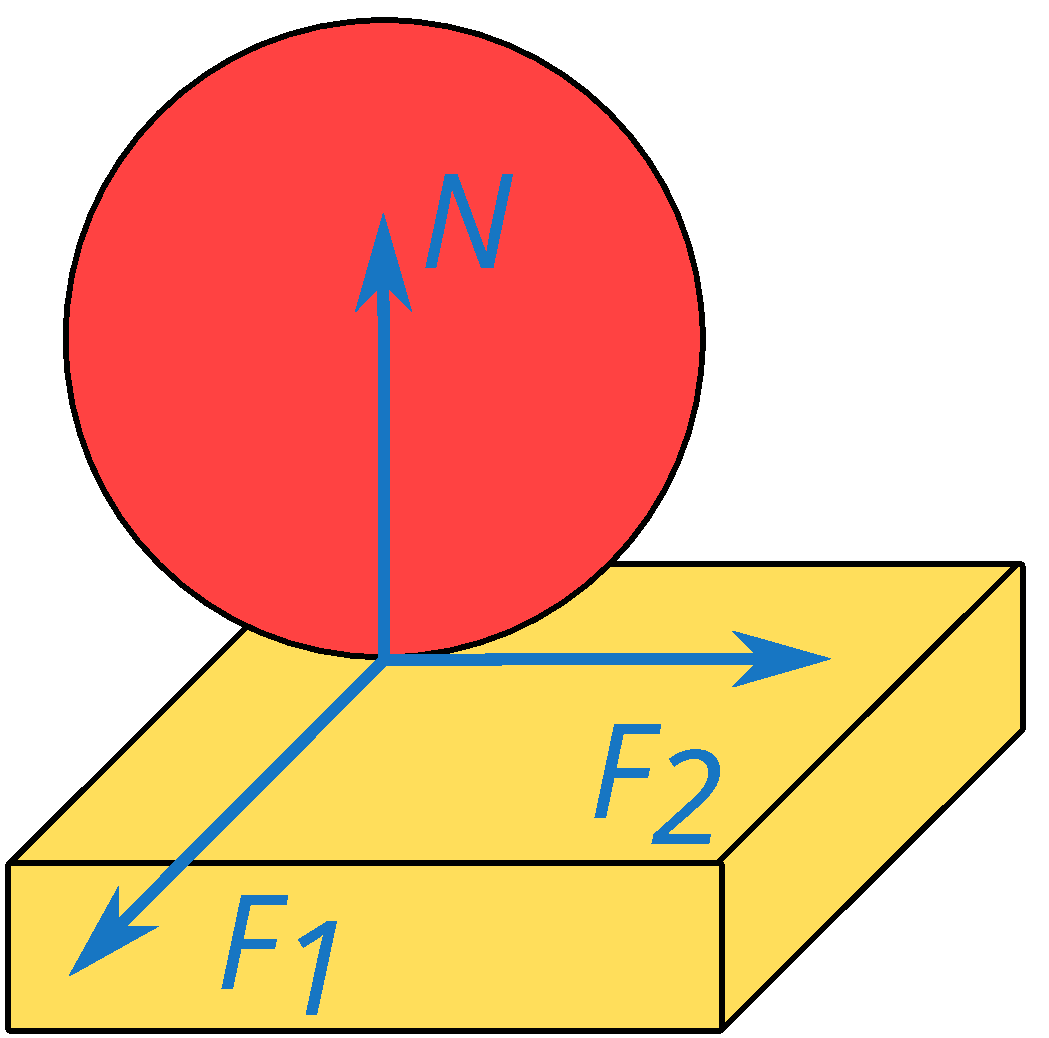
\includegraphics[width=0.5\textwidth]{graphics/friction.pdf}
		\caption{Wersory punktu kolizji.}
		\label{fig:ode_collision}
		\end{figure} 

		Po wykryciu punktu kolizji i wyznaczeniu wektora normalnego $N$ do dotykających się obiektów, system powinien obliczyć odpowiednie wartości sił, 
		aby zatrzymać lub odbić obiekty od siebie.
		Dodatkowo, ponieważ prędkości obiektów nie muszą być równoległe do $N$, należy zasymulować siłę tarcia z odpowiednią dla współczynnika tarcia wartością.
		Można to uzyskać, nadając obiektom w punkcie kolizji siłę $F$ prostopadłą do $N$, 
		ten wektor może być rozpisany przy pomocy dwóch wektorów jednostkowych $f_0$ i $f_1$. 
		Te wektory zawsze są prostopadłe do $N$, równoległe do płaszczyzny kolizji.

		W standardowej symulacji fizyki nigdy nie potrzeba osobno modyfikować współczynników tarcia i kierunku tych wektorów, 
		gdyż zazwyczaj powierzchnie symulowanych obiektów mają jednakowe współczynniki tarcia w każdym kierunku.
		Jednakże modyfikując te wektory statycznie, lub dynamicznie, można uzyskać bardzo interesujące efekty.
		Instrukcja silnika symulacji podaje przykład, w którym aby zamodelować tarcie opon samochodu na zakręcie, prostopadle do kierunku jazdy, 
		należy dynamicznie zmieniać współczynnik tarcia dla wektora $f_0$, lub $f_1$ w kierunku promienia koła.
		Ten współczynnik tarcia, prostopadły do kierunku jazdy, może być liniowo zależny od prędkości.
		Spowoduje to, że im większa prędkość samochodu, tym boczna siła odśrodkowa bardziej wpłynie na tor jego jazdy, co ma odwzorowanie w rzeczywistości.
		Więcej informacji można znaleźć na stronie instrukcji maszyny symulacyjnej ODE \cite{ode_contact}.

		W opisywanym tutaj modelu, modyfikuje się wektor $f_0$, oraz współczynniki tarcia dla obu wektorów, aby przybliżyć zachowanie się rolki.
		Ponieważ wektory $f_0$ i $f_1$ są określone w lokalnym dla koła układzie współrzędnych, 
		w każdej iteracji maszyny symulacji należy obrócić je względem aktualnej pozycji bazy i odwrotności obrotu koła.
		Idealna rolka obraca się całkowicie bez tarcia, a ruch równolegle do jej osi jest niemożliwy.
		Można więc ustawić zerowy współczynnik tarcia w kierunku prostopadłym do osi, oraz nieskończenie duży dla wektora równoległego do osi.

		\begin{figure}[h]
		\centering
		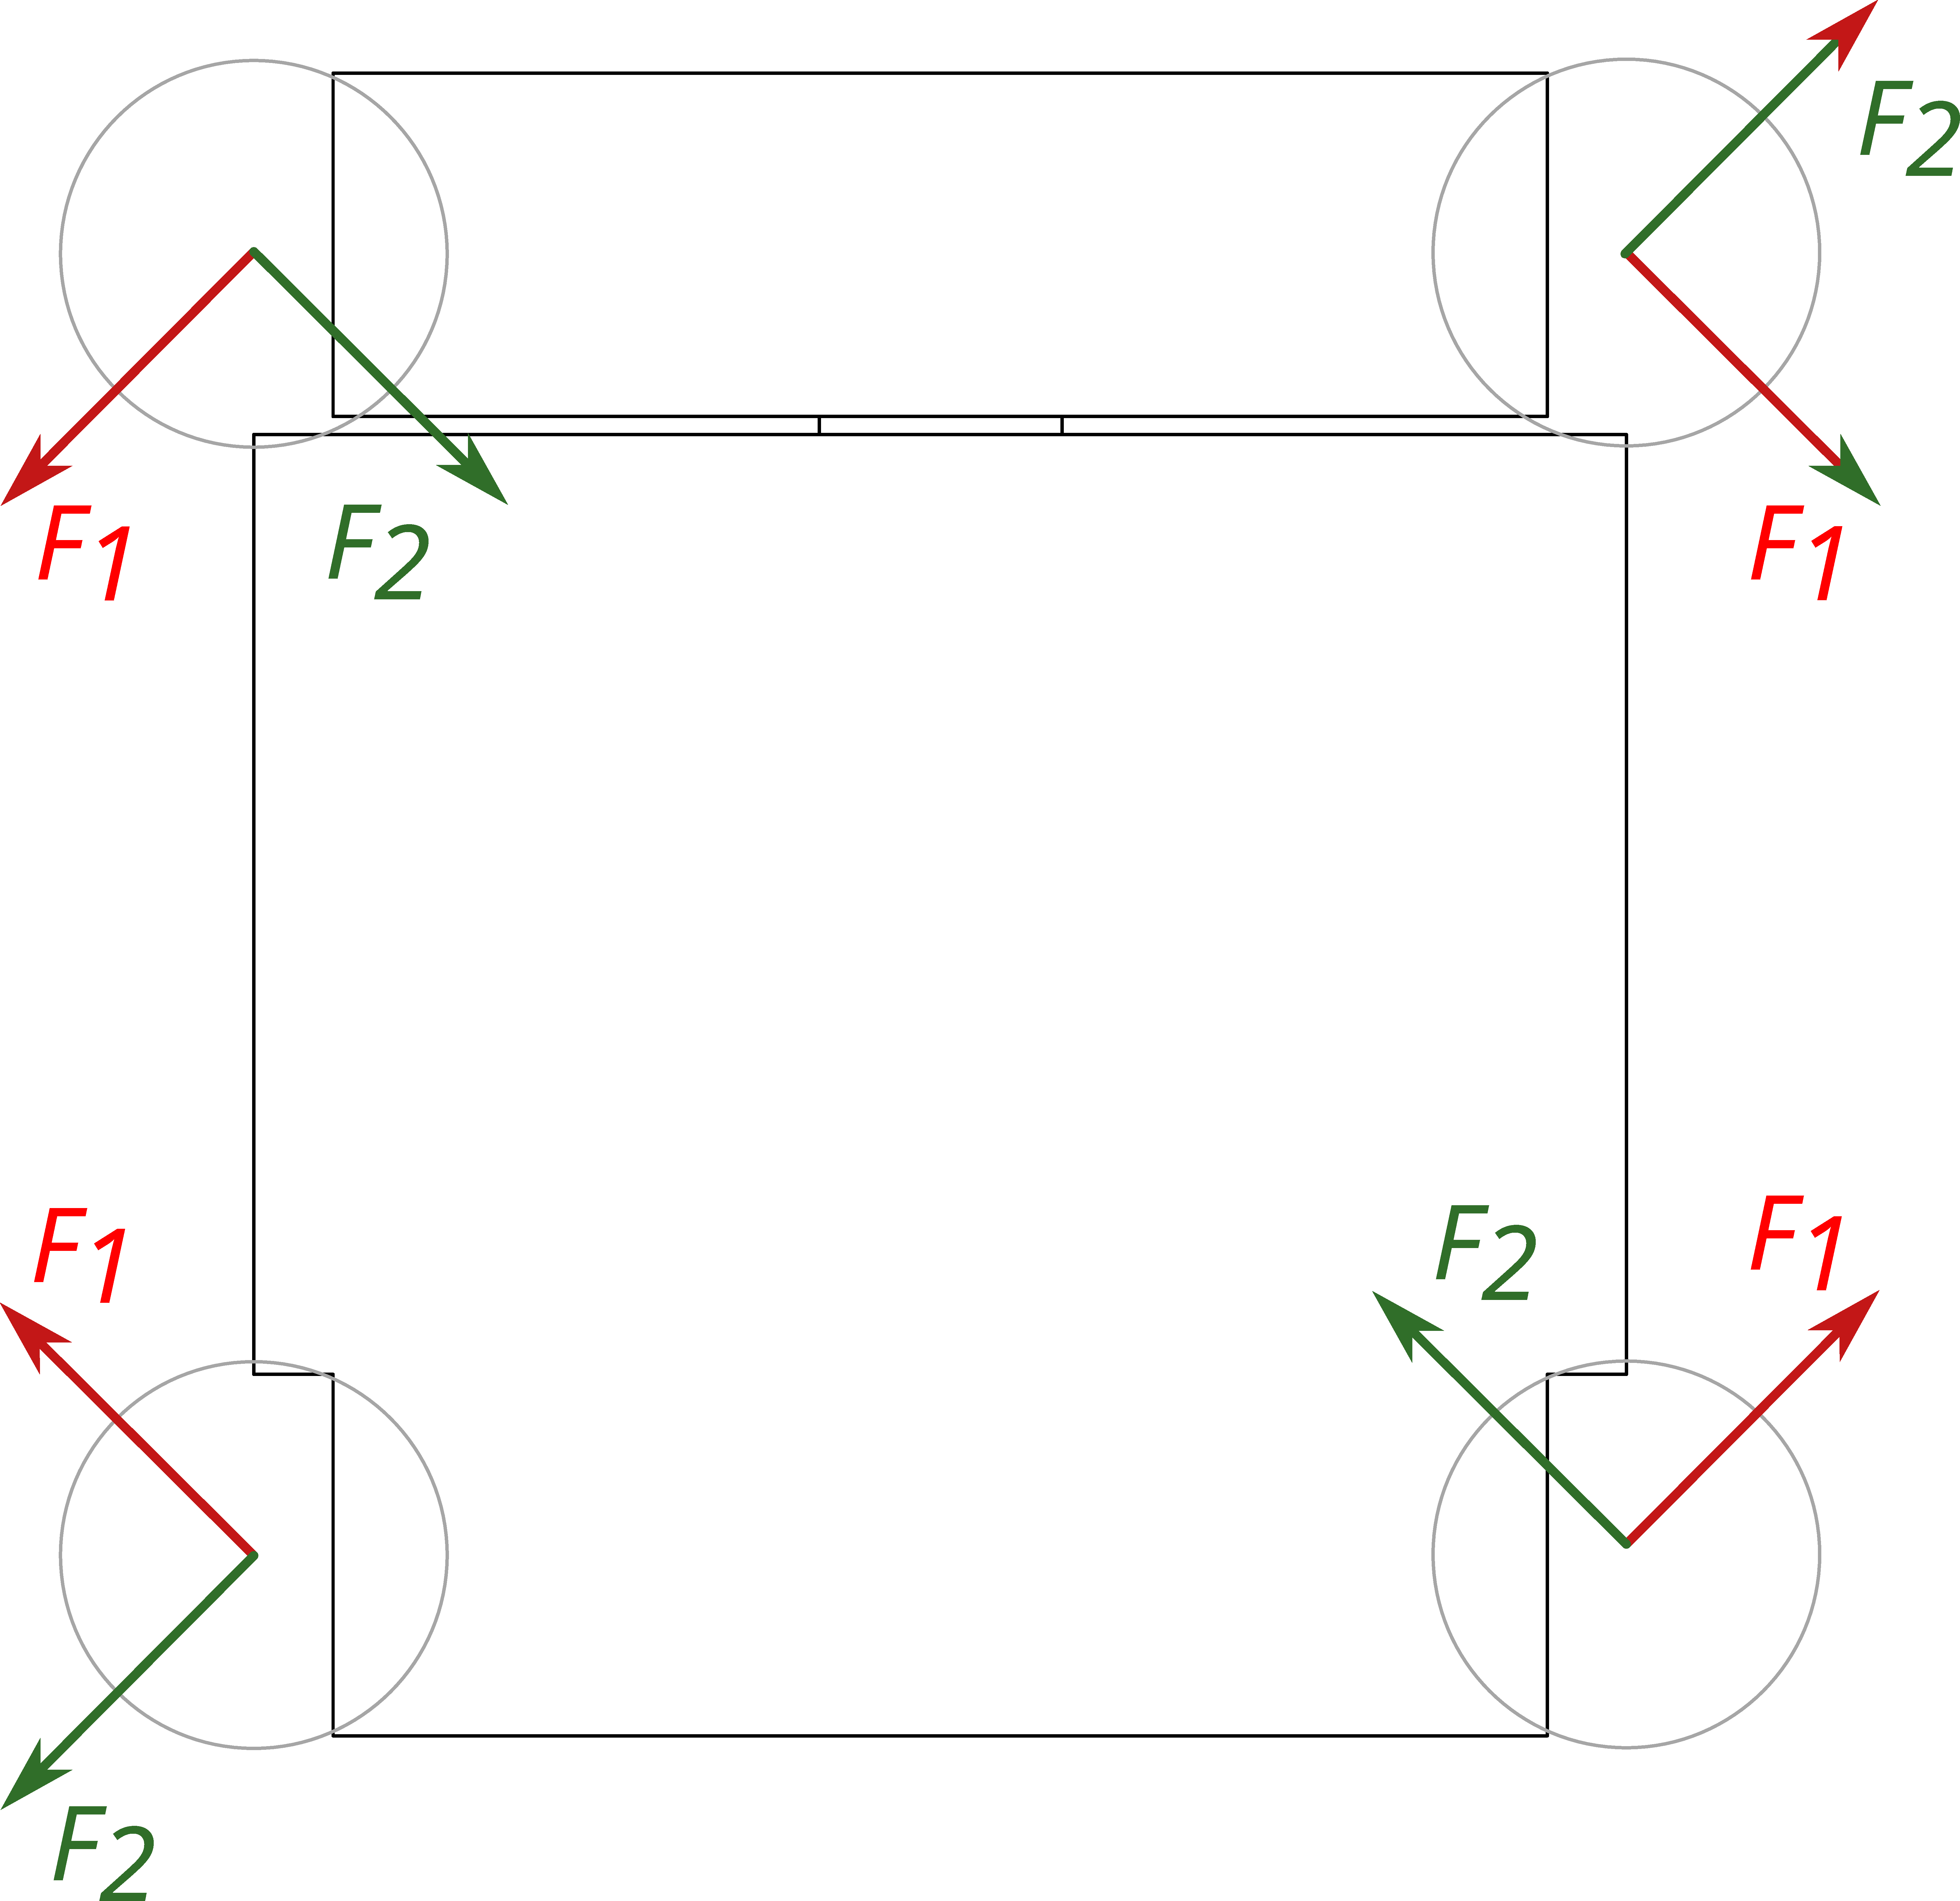
\includegraphics[width=0.6\textwidth]{graphics/base_vects.pdf}
		\caption{Kierunki wektorów dla których należy nadać współczynniki tarcia przy symulacji platformy, widok z góry. Tarcie w kierunku $f_0$ powinno być nieskończone, a w $f_1$ zerowe.}
		\end{figure} 

		Niestety, w rzeczywistości rolki wykonane są ze śliskiego plastiku, który zezwala na poślizg kół wzdłuż ich osi.
		Osie kolek również nie obracają się płynnie, trzeba użyć dużej siły, aby obrócić dowolną z nich, pod naciskiem platformy tarcie jest jeszcze większe.
		Każda rolka obraca się z innym tarciem wprowadzając kolejne zakłócenia.
		Podłoże po którym porusza się robot także nie jest tu bez znaczenia.
		Należy zatem wystawić interfejs do łatwej zmiany współczynników tarcia, aby później dobierać odpowiednie wartości na podstawie zachowania rzeczywistego robota.

		Podobnie, jak w poprzednich przypadkach, modeluje się tylko najniższą, dotykającą podłoża rolkę.
		Jak wcześniej wspomniano, ma ona bardzo skomplikowany kształt, lecz można przybliżyć całe koło kulą.
		Zatem w miejscu każdego koła ustawiona jest kula z dynamicznie modyfikowanym tarciem i siatką trójkątów w kształcie koła do wizualizacji, 
		oraz przegub z motorem łączący odpowiednią część bazy z kołem.
		To najprostsza budowa modelu (a zatem najszybsza) z poprzednich.
		
		\begin{figure}[H]
		\dirtree{%
		.1 korpus\DTcomment{Podstawa bazy}.
		.2 przegub obrotowy\DTcomment{Nadaje moment obrotowy}.
		.3 kula\DTcomment{Modyfikowane wektory tarcia}.
		.3 siatka trójkątów\DTcomment{Odpowiada za wizualizację koła}.
		}
		\caption{Logiczne zagnieżdżenie obiektów koła w strukturze drzewiastej z modyfikowanymi wektorami tarcia. W implementacji Gazebo przegub i kula są ustawione równolegle.}
		\label{fig:omnivelma_wheel}
		\end{figure}

		Takie rozwiązanie wiąże się z pewnym ryzykiem.
		Wymaga, aby symulator używał maszyny ODE, co zmniejsza przenośność modelu. ODE jest domyślnym symulatorem w Gazebo.
		Maszyna Bullet również liczy kolizje w ten sposób i ma modyfikowalne wektory, 
		lecz nie daje podobnych wyników. Być może jest to spowodowane brakiem odpowiedniej konfiguracji, lub innym wewnętrznym traktowaniem modelu.
		
	\subsection{Ustawienie mas i momentów bezwładności}
		W standardzie SDF zdefiniowano element \texttt{inertial}, który definiuje w sobie masę oraz macierz inercji. 
		Dla uproszczenia wszystkie ogniwa mają ustawione swoje środki w punktach środków mas, co oznacza, że każda z macierzy inercji jest macierzą przekątną.
		Masy zostały nadane zgodnie z danymi z tabeli \ref{tab:masses}, a macierze inercji obliczone ze wzorów na macierze inercji prostopadłościanu lub walca.
		Gazebo pozwala na wizualizację nadanych parametrów w formie narysowanych prostopadłościanów.
		
		Środki mas zostały obliczone, bazując na uproszczonych kształtach ogniw, przy założeniu jednorodnego rozkładu gęstości w korpusie.
		
		Jeśli dane mas i momentów bezwładności nie są logicznie ustawione, lub zostawione na domyślnych wartościach, model może powodować błędy maszyny symulacyjnej.
		Występują wtedy ,,glitche'', czyli losowy ruch i obrót obiektu w różnych kierunkach. Model wpada w taki stan i leci w losowym kierunku. 
		Taki efekt czasami występuje w grach komputerowych. Jest to spowodowane tym, że dochodzi do błędów obliczeń numerycznych z powodu za dużych różnic w parametrach obiektów
		i obliczeń kolizji.
		
	\subsection{Model silników}
		Platforma wyposażona jest w cztery niezależne serwomotory. 
		Model takiego obiektu jest przegubem obrotowym, któremu należy nadawać odpowiednią prędkość, w zależności od odebranych pakietów.
		Ponieważ każda maszyna symulacyjna fizyki inaczej interpretuje tę wartość, należy zwrócić szczególną uwagę na sposób nadawania prędkości obiektom.
		
		Przede wszystkim, prędkość jest zawsze reakcją na przyłożoną siłę lub moment obrotowy. W rzeczywistości nie istnieje sposób na natychmiastowe nadanie prędkości obiektowi.
		Pomimo że maszyna posiada wewnętrzną informację o aktualnej prędkości,
		jej bezpośrednia modyfikacja może wprowadzać nietypowe zachowania. Przede wszystkim należy brać pod uwagę reakcję ze strony połączonego obiektu, w tym przypadku korpusu,
		a także czasu nadania tej prędkości. Powinna być zsynchronizowana z krokami symulacji a nie częstotliwością odbioru wiadomości ze strumienia.
		
		Najlepsze efekty daje nie nadawanie prędkości obiektom, a nadanie docelowej prędkości i maksymalnego momentu obrotowego.
		Maszyna symulacji fizyki wtedy odpowiednio zinterpretuje dane, obliczając również reakcję na obu końcach przegubu.
		Jest także możliwość ustawienia algorytmu sterownika, na przykład PID, ale takiemu należy także nadać odpowiednie parametry do pracy.
		
		W modelu odwołano się bezpośrednio do zmiennych maszyny symulacyjnej ODE za pomocą interfejsu symulatora Gazebo.
		Jest to metoda wirtualna, implementowana do komunikacji z każdą maszyną symulacyjną osobno.
		\begin{minted}{cpp}
virtual bool SetParam (const std::string& key,
	unsigned int index,
	const boost::any& value)
		\end{minted}
		Metoda przyjmuje nazwę modyfikowanej wartości, oś przegubu (dla silników to zawsze będzie jedyna oś \texttt{0}) oraz nadawaną wartość.
		Modyfikowane wartości to:
		\begin{description}
			\item[\texttt{fmax}] Maksymalny moment obrotowy w \si{\newton\metre}, używany przez maszynę symulacyjną do nadania docelowej prędkości kątowej przegubowi. Ustawiany raz przy inicjalizacji modelu. Ponieważ w platformie ta wartość nigdy nie będzie osiągnięta ze względu na ograniczenia energetyczne, można założyć tutaj wysoką liczbę 100 \si{\newton\metre}.
			\item[\texttt{vel}] Docelowa prędkość obrotowa w \si{\radian\per\second} zapamiętana i ustawiana w każdym kroku symulacji, nadpisywana na odbiór nowych wartości z komunikacyjnego strumienia wiadomości.
		\end{description}
	
	\subsection{Komunikacja}
		Ze względu na wiele ustawień elementów bazy, należy stworzyć bogaty interfejs.
		W każdym cyklu symulacji, program sterujący modelem platformy nadaje wiadomości:
		\begin{itemize}
		\item \texttt{geometry\_msgs/PoseStamped} z aktualnym położeniem i orientacją platformy, oraz nagłówek z czasem i identyfikatorem.
		\item \texttt{geometry\_msgs/TwistStamped} z aktualną prędkością platformy i nagłówkiem.
		\item \texttt{omnivelma\_msgs/EncodersStamped} z odczytaną ze stanu obiektów kół aktualną prędkością kątową i kątem obrotu, z nagłówkiem. 
		To jest symulator enkoderów wbudowanych w silniki platformy.
		\end{itemize}
		
		Przyjmowane są także dane:
		\begin{itemize}
		\item \texttt{omnivelma\_msgs/Vels} z zadanymi prędkościami kół.
		\item Wywołanie ustawiające współczynniki tarcia wzdłuż wektorów $f_0$ i $f_1$.
		\item Wywołanie ustawiające masy i momenty obrotowe niektórych elementów składowych konstrukcji.
		\end{itemize}

	\subsection{Rozszerzenie modelu}
		\label{sec:model_nan}
		Ponieważ komputerowa reprezentacja liczby zmiennoprzecinkowej pozwala na zapisanie nie tylko liczbowych wartości, można rozszerzyć model o dodatkową funkcjonalność,
		wywoływaną wysłaniem do modelu cichej nie-liczby (\emph{NaN}) w wiadomości, w polu prędkości odpowiedniego koła. 
		Cicha nie-liczba powstaje w procesorze, w module operacji zmiennoprzecinkowych, przy przeprowadzaniu nieprawidłowych, 
		acz niekrytycznych obliczeń, na przykład dzielenie przez zero, lub dzielenie nieskończoności przez minus-nieskończoność 
		(także zapisywane jako forma liczby zmiennoprzecinkowej).
		Takie operacje nie powodują błędu programu, jedynie wynik w postaci nie-liczby propaguje przez wszystkie pozostałe operacje.

		Nadanie prędkości modelom w przestrzeni wirtualnej polega na wywołaniu odpowiedniej funkcji maszyny symulującej fizykę.
		Można zadać pytanie, jak zachowa się model, jeśli dla niektórych kół nie zmieniać prędkości po każdym odebraniu pakietu?

		Wobec tego, jeśli w pakiecie z nowymi prędkościami kół znajdzie się cicha nie-liczba, program sterujący nie nada nowej prędkości temu kołu.
		Jest to podobne do nadania tej samej prędkości, jaką posiada aktualnie obiekt koła (jaką zwróciłby enkoder).

		Zwraca to uwagę również na potrzebę, aby program do komunikacji z rzeczywistym robotem nie skończył się błędem po odebraniu jednej z takich nieokreślonych wiadomości.
		Ponieważ przekształca liczby zmiennoprzecinkowe, zawarte w ROSoswych pakietach, na dane zrozumiałe przez sterownik silnika, które zazwyczaj są liczbami
		stałoprzecinkowymi, program może zachować się nieprzewidywalnie.
		
\section{Model skanera laserowego}
	Ponieważ skanery laserowe tego typu są popularnie używane w robotyce, standard SDF posiada dedykowane elementy do umieszczenia takich obiektów w symulacji.
	Również Gazebo posiada możliwość renderowania zasymulowanych impulsów lasera.
	
	\subsection{Obliczenia symulatora}
		Skaner laserowy jest bardzo łatwo zasymulować w przestrzeni wirtualnej za pomocą rzutowania półprostych.
		Ta technika używana jest w bardzo wielu aspektach komputerowego generowania obrazu i symulacji fizyki.

		Półprosta jest emitowana z ustalonego punktu w pewnym kierunku w przestrzeni trójwymiarowej.
		Następnie system próbuje znaleźć pierwszy punkt jej kolizji z każdym z obiektów o fizycznym kształcie, uczestniczących w symulacji.
		
		Ponieważ zasoby komputera zawsze są ograniczone, długość promienia także musi mieć pewien limit. 
		Zwykle jest on jednak na tyle duży, że z punktu widzenia obiektów uczestniczących w symulacji, w opisywanym tutaj zagadnieniu, 
		można uznać tą odległość za nieskończoną.

		Algorytm obliczania kolizji z półprostą bazuje na kosztowym porównywaniu pozycji każdego obiektu fizycznego na scenie.
		Istnieją oczywiście sposoby na zmniejszenie ilości obliczeń, na przykład metoda prostopadłościanów zawierających obiekt, ale sposób radzenia sobie z tym zagadnieniem nie jest
		częścią tematu pracy,
		Wystarczy wspomnieć, że symulacja dużej ilości laserów oraz obiektów jest operacją kosztowną.
		
		Testy pokazują, że samo ich rysowanie spowalnia symulację około czterokrotnie.
		To ze względu na bardzo dużą ich ilość, mogącą przekroczyć 1000 obliczeń kolizji w jednej klatce symulacji.

	\subsection{Różnice między czujnikiem, a modelem}
		Półprosta emitowana jest z puntu reprezentującego środek skanera.
		Model upraszcza rzeczywisty czujnik (budowa skanera laserowego została opisana w sekcji \ref{sec:lidar}).
		Uproszczenie to polega na tym, iż nie ma wewnątrz zamodelowanego obiektu żadnego odpowiednika obracającego się lusterka.
		W rzeczywistym czujniku ponadto jest jeden laser, emitujący pulsy w określonych odstępach czasu.
		W modelu warto zatem emitować osobne półproste, dla każdego pulsu lasera.

		Można zauważyć tym samym, że model skanera wydaje się funkcjonalnie lepszym, niż rzeczywisty LiDAR.
		W danej chwili, model emituje promień we wszystkich kierunkach w zakresie jednocześnie, podczas gdy skaner jednym pulsem może dokonać tylko jednego pomiaru,
		i tylko o kącie w którym aktualnie znajduje się lusterko.
		Jednakże dyskretny sposób symulacji i sposób komunikacji urządzenia z odbiornikiem danych, powodują że w obu przypadkach dane są podawane w grupach.
		Sterownik skanera jest wstanie wysłać pakiet z danymi z ostatniego pomiaru, podczas gdy program modelujący skaner jest obsługiwany na zasadzie przerwań czasowych 
		po każdym kroku symulacji i tylko wtedy może wywołać funkcje zwracające dane zasymulowanych pomiarów.
		To oznacza, że interfejsy do ich obsługi zachowują się podobnie.

		Drugą rzeczą, w której model przoduje, jest nieskończona (z punktu widzenia symulacji), odległość pomiaru.
		Nie tylko jako najdalszy wykryty punkt, ale także i najbliższy. 
		Skaner może pomijać pomiary przypadające za blisko krawędzi dozwolonego obszaru, gdyż znacznie spada w tych miejscach dokładność pomiaru, lub zwracać niedokładne dane.
		Symulator ma całkowitą dowolność w ustawianiu progu, dla którego obcina pomiar.

		Podobnie, jak w poprzednim przypadku, symulator posiada niezmienną w odległości dokładność pomiaru.
		Błąd pomiarowy sknera laserowego zależy od odległości od mierzonego obiektu.

		Jednakże, w zależności od obciążenia maszyny na której uruchomiony jest symulator, model skanera jest podatny na opóźnienia w odczytywaniu stanu.
		Skaner zawsze działa z tą samą częstotliwością, a jego program sterujący jest wbudowany w mikrokontroler i spełnia sztywne ramy czasowe.

	\subsection{Komunikacja}
		Bazując na architekturze opisanej wcześniej na rysunku \ref{fig:agent}, należy tak zbudować system, aby program sterujący mógł się komunikować w identyczny sposób z 
		modelem skanera, jak i samym skanerem.
		Służą do tego specjalne typy wiadomości ROSa \texttt{sensor\_msgs/LaserScan}.
		Program obsługujący model skanera generuje i wysyła pakiety zawierające:
		\begin{itemize}
			\item Nagłówek z czasem pomiaru, numerem sekwencyjnym i identyfikatorem macierzy przekształcenia jednorodnego pozycji czujnika.
			\item Kąty początkowe i końcowe pomiaru.
			\item Odległość kątowa pomiędzy kolejnymi promieniami.
			\item Czas pomiędzy kolejnymi emisjami lasera.
			\item Czas pomiędzy tym, a poprzednim przebiegiem urządzenia.
			\item Minimalny i maksymalny dystans mierzonego obiektu od skanera.
			\item Dane odległości.
			\item Dane jasności (jeśli czujnik posiada taką funkcjonalność).
		\end{itemize}

		Identycznie, program podłączony bezpośrednio do skanera za pomocą jednego z interfejsów, także powinien generować takie same pakiety i udostępniać je w środowisku ROS.
		
	\subsection{Model w Gazebo}
		Tak, jak w modelu platformy, należy stworzyć odpowiedni plik SDF. 
		Warto umożliwić stosowanie modelu czujnika w modelach innych robotów. 
		Zatem jego implementacja powinna być niezależna od implementacji platformy, do której będzie przytwierdzony.
		Dodatkowo, w końcowym modelu istnieć będą dwa takie czujniki, budowa pliku powinna pozwolić na wielokrotne importowanie tych samych danych do tego samego modelu, 
		ale jednak aby były interpretowane w różny sposób (gdyż nadawcy danych muszą być rozróżnialni).

		Model składa się z dwóch elementów: korpusu i samego ,,mechanizmu'' urządzenia.
		Mechanizm przytwierdzony jest w odpowiednim miejscu korpusu platformy, za pomocą stałego przegubu (elementu \texttt{joint}).

		Korpus czujnika posiada siatkę trójkątów, reprezentującą uproszczony wygląd urządzenia, a także dwa elementy ustawiające walcowate kształty, odpowiedzialne za kolizje fizyczne.
		Teoretycznie, lepiej było by, gdyby model posiadał jeden walec, reprezentujący kształt urządzenia, gdyż to przyspieszyłoby symulację. 
		Jednakże, półproste emitowane ze środka obiektu, również się by z nim zderzały od wewnątrz, a co za tym idzie, nie opuszczałyby modelu czujnika.
		Element korpusu odpowiada także za przesunięcie samego lasera względem podstawy, na której całe urządzenie jest montowane, i 
		pozwala na wygodną referencję z innego modelu, w celu utworzenia przegubu.
		Jak już wcześniej wspomniano, model zawsze ma strukturę gwiazdową i przeguby po stronie robota nie mogą wskazywać na element \texttt{model} modelu skanera, a mogą
		na obiekt korpusu.

		Główna część obiektu czujnika, skaner, posiada ozdobną siatkę trójkątów, udającą czarną szybkę LiDARa, oraz element SDF \texttt{sensor}, odpowiedzialny za sam czujnik.
		W kolejnych podelementach zawierają się parametry urządzenia, takie jak ilość symulowanych laserów, ich zasięg, kąt pierwszego i ostatniego lasera, oraz współczynnik błędu pomiarowego. Ten element celowo nie ma fizycznego kształtu, aby nie blokować wychodzących półprostych. 
		Nie wpływa to na symulację, gdyż w środowisku, w którym znajduje się robot, i tak nie powinno dochodzić do kolizji modeli czujników z jakimikolwiek innymi modelami.
		Również czujniki nie są wstanie wykryć siebie nawzajem, gdyż zwrócone są do siebie martwymi kątami, a co za tym idzie nie muszą symulować nieprzezroczystych brył dla
		innych sensorów.
		W przeciwnym wypadku, element fizycznego kształtu pośrodku urządzenia byłby wymagany.

		\subsubsection{Połączenie modeli}
			Jak wcześniej wspomniano w sekcji \ref{sec:sdf},
			model SDF ma strukturę gwiaździstą. 
			Zagnieżdżenie modeli spowodowałoby, że powstałaby inna struktura, drzewiasta.
			Dlatego też, element \texttt{import} nie umieszcza w swoim miejscu całego modelu z innego pliku, a raczej importuje jego ogniwa i umieszcza równolegle do istniejących.
			To oznacza, że zadbać trzeba także o więzy \texttt{joint}, łączące element podstawy platformy z podstawą czujnika, inaczej symulator uznałby łączony obiekt za dwa osobne modele.
			Potrzebna jest zatem znajomość nazw elementów ogniw importowanego modelu.
			Element \texttt{model} importowanego modelu jest tracony, pozostaje jedynie przedrostek nazwy w zaimportowanych składowych.
			Zatem program sterujący czujnikiem powinien na podstawie tylko nazwy swojego obiektu ustawić przedrostek swojego interfejsu nadawania wiadomości.

			Taka mechanika działania wydaje się mało zrozumiała i nieintuicyjna, jednak doskonale dba o zachowanie spójności modelu.
			Wszystko nadal pozostaje strukturą gwiaździstą i każdy element musi być odpowiednio połączony z pozostałymi, aby dokładnie określić fizykę interakcji.
			Nie powstają niedopowiedziane sytuacje, w których zachowanie jakichś ogniw byłoby nieokreślone.

			Alternatywnie, zawsze jest możliwość stworzenia dwóch, osobnych modeli skanerów, tudzież całość zapisać w jednym pliku.
			Jednak takie rozwiązanie niszczy pakietową budowę środowiska i nie pozwala na użycie modeli skanerów w innych modelach.
			
			Należy zadbać o ustawienie odpowiedniej struktury macierzy przekształceń jednorodnych, opisanej w sekcji \ref{sec:frames}.
			Symulator platformy zawiera drugi program, który w każdym cyklu symulacji nadaje demonowi ROS położenia i orientacje środków czujników laserowych, dla uproszczenia
			względem początku układu współrzędnych, punktu (0,0,0). 
			Program sterujący modelem samej platformy także nadaje przekształcenie z pozycją platformy względem globalnego środka układu współrzędnych.
			Dokładnie taki sam efekt byłby, gdyby nadawać przekształcenie ze stałą pozycją czujników laserowych, ale względem platformy (której przekształcenie nadawane jest przez inny sterownik).
			Stałą pozycją, ponieważ czujniki nie zmieniają swojej pozycji na platformie, są przytwierdzone na stałe.

	\subsection{Błędy}
		Jak podano wcześniej w tabelce \ref{tab:lidar}, wyróżnione są dwa typy błędów pomiaru, systematyczny i pomiarowy.
		Dodatkowo istnieje także błąd gruby.
		Model czujnika powinien uwzględniać wszystkie błędy, aby zwracać dane jak najbardziej zbliżone do LiDARa.

		\subsubsection{Błąd gruby}
			Najprostszy typ błędu polega na dużych odchyłach niektórych pomiarów od pozostałych wartości.
			W trakcie przetwarzania odczytu, te punkty powinno się odrzucić.
			Pomimo, że sterownik skanera usuwa takie błędy, można łatwo dodać je do generowanych danych w celu testowania algorytmów określania pozycji.

			Najczęstszym przypadkiem błędu grubego jest brak odbioru wysłanego impulsu. 
			To skutkuje nadaniem aktualnemu pomiarowi wartości maksymalnej, co jest bardzo łatwo wykryć i usunąć.

			Innym problemem może być odebranie światła niepochodzącego od emitera urządzenia, a jakiegoś zewnętrznego źródła.

			Ponieważ rozkład i częstotliwość tych błędów zależy od środowiska w jakim działa czujnik, bardzo ciężko jest dobrać odpowiedni algorytm ich generacji.

		\subsubsection{Błąd systematyczny}
			Ten błąd jest stałą wartością, dodaną do każdego pomiaru.
			Spowodowany jest niedoskonałością budowy elementów pomiarowych, niewłaściwą kalibracją, zużyciem, lub otoczeniem w jakim pracuje czujnik.

			Rzeczywisty LiDAR powinien być skalibrowany przed użyciem właśnie po to, aby wewnętrzny program sterujący mógł obliczyć aktualne zboczenia pomiarów
			i skorygować dane przed wysłaniem ich wyżej.
			Skaner może także wysyłać czyste i obarczone błędami dane do programu sterującego, który samodzielnie je skoryguje.
			Pozwoli to na zastosowanie dowolnych algorytmów oczyszczania danych, kosztem większego obciążenia programu sterującego.

			Symulator czujnika nie nie jest podatny na takie błędy, więc nie ma sensu dodawać interfejsu do kalibracji urządzenia.
			Można co najwyżej symulować niepoprawnie skalibrowany skaner poprzez sztuczne dodanie takiego błędu.

		\subsubsection{Błąd pomiarowy}
			Jest to mała, losowa wartość, dodana do każdego pomiaru.
			Wynika ona z niedoskonałości samego czujnika, nieznanych zakłóceń i niezbadanych efektów kwantowych.
			Nie da się w żaden sposób usunąć, zmniejszyć, lub przewidzieć tego typu błędów.
			Jedynym sposobem jest obliczenie średniej błędu na podstawie dużej ilości pomiarów.

			Błąd pomiarowy ma zwykle rozkład normalny o określonym odchyleniu standardowym.
			Standard SDF przewiduje element określający tę liczbę, a Gazebo może wewnętrznie obliczyć i dodać do wyników odpowiednią wartość.
			Również producent podał w tabeli danych urządzenia obliczony rozkład standardowy.

			W związku z tym, wartość podana przez producenta, podana w tabelce \ref{tab:lidar}, może być bezpośrednio zapisana do 
			elementu odchylenia standardowego, w pliku SDF opisującym czujnik.
			Wadą takiego rozwiązania jest niemożność modyfikacji tego parametru w trakcie wykonywania programu, gdyż Gazebo nie wystawia API do modyfikacji tej wartości.
			Aby temu zaradzić, wystarczy obliczać błąd standardowy w programie sterującym i manualnie dodawać go do zwróconej przez symulator tablicy danych.
			Funkcje do obliczania błędu standardowego zostały wprowadzone do standardu języka C++.
			
			Na zrzucie ekranu \ref{fig:scan} można zobaczyć, iż punkty pomiarów, wizualizowane w RViz, nie leżą idealnie na figurach powstałych poprzez przecięcia skanowanych brył.
			Dodany jest szum, jak gdyby rozmazujący punkty.
		
\section{Model jednostki inercyjnej}
	Ponieważ czujniki tego typu są często stosowane w robotyce, ROS i Gazebo wspierają jego symulację i struktury przekazywanych danych.
	\begin{itemize}
		\item ROS posiada specjalną wiadomość typu \texttt{sensor\_msgs/Imu}, do przekazywania pomiarów pomiędzy węzłami.
		\item SDF definiuje element typu \texttt{imu} w sekcji czujników, gdzie można mu zdefiniować położenie w robocie i współczynniki błędów pomiarowych.
		\item Gazebo daje wsparcie klasy czujnika inercji z odczytem wygenerowanych przez maszynę symulacji wartości.
	\end{itemize}
	
	Warto tutaj nadmienić, że struktura wiadomości ROSa posiada pola dla danych, które nie koniecznie mogą być wygenerowane przez czujnik rzeczywisty.
	Takimi polami jest struktura rotacji, zapisana jako kwaternion, oraz macierze kowariancji, wyznaczane zewnętrznie eksperymentalnie.
	
	Macierze kowariancji definiują wpływ danych z jednej osi na drugą i mnożniki wyjścia. 
	Nierówność pomiarów na przykład może być to spowodowana odchyleniem akcelerometrów względem kąta prostego, co powoduje że ruch w osi jednego czujnika może
	być także wykryty przez czujniki innych osi. 
	Podobnie jest, gdy czujniki nie generują dokładnie tych samych danych na taki sam ruch wzdłuż ich osi, co może być spowodowane niedokładnością wykonania elementów.
	Macierz pozwala zastosować te cechy sprzętowe do danych w celu poprawy ich jakości.
	
	W większości programów używających przestrzeń wirtualną, rotację zapisuje się w postaci kwaterniona, jako cztery liczby.
	Taka postać odporna jest na zjawisko utraty jednego ze stopni swobody (\emph{gimbal lock}). Gdy dwie z trzech osi pokryją się, niemożliwy staje się obrót obiektu wokół trzeciej osi. Niestety, taka postać rotacji nie ma odwzorowania w rzeczywistej przestrzeni.
	
	Symulacja żyroskopu w maszynie symulacyjnej fizyki jest bardzo prosta, gdyż algorytm wyznaczania pozycji obiektów na podstawie nadanych sił korzysta wewnętrznie z
	wartości prędkości dla każdego obiektu. Zatem kwestia symulacji tego sensora polega na odczycie odpowiednich struktur z maszyny symulacji.
	Wtyczka do Gazebo, zapisana podobnie do wtyczki czujnika laserowego, zbiera w każdym cyklu maszyny symulacyjnej dane i wysyła ja za pomocą pakietu ROSa.
	
	Na podstawie testu opisanego w sekcji \ref{sec:test_ang}, wyznaczono w tabeli \ref{tab:imu_noise} parametry dodatkowego szumu, dodawanego do odczytów w celu dokładniejszego zamodelowania błędów pomiarowych.
	
	\begin{table}
		\centering
		\begin{tabular}{l r}
		Opis & Wartość \\
		\hline
		Średnia					&	0 \\
		Odchylenie standardowe	&	0,003 \si{\radian\per\second} \\
		\end{tabular}
		\caption{Wartości szumu o rozkładzie Gaussa, zastosowanego w modelu czujnika prędkości kątowej.}
		\label{tab:imu_noise}
	\end{table}
	
	Akcelerometr jest bardziej złożonym problemem, gdyż maszyna symulacji działa w czasie dyskretnym, co utrudnia różniczkowanie prędkości w celu otrzymania przyspieszenia.
	Ta wartość nie jest także nigdzie indziej używana i musi być obliczona specjalnie dla symulacji tego czujnika.
	Fakt, że małe odchylenia w zmianie prędkości powodują duże skoki danych przyspieszenia, wprowadza naturalny szum do generowanych danych.
	W sekcji \ref{sec:test_imu}, opisane zostały te problemy dokładniej.
	
	Pomimo, że odczytanie tych wartości jest tak samo proste, jak prędkości kątowej, to generowane dane różnią się jakością.
	Szum jest większy, a co za tym idzie, potrzeba dodatkowego programu do odszumienia wygenerowanych wartości.
	Ten pakiet jest opisany w sekcji \ref{sec:odszumiacz}.
	
\section{Manualne sterowanie}
	\subsection{Program}
		Ten pakiet jest plikiem wykonywalnym, skompilowanym ze źródeł w C++, w sposób opisany w sekcji \ref{sec:ros_exe}.
		Wykorzystując bibliotekę graficzną SFML, generuje okno z powierzchnią do rysowania na nim za pomocą OpenGL.
		Biblioteka ta pozwala również na bezproblemowe przechwytywanie zdarzeń z klawiatury, takich jak wciśnięcie i puszczenie klawisza, a także na obsługę kontrolera go gier i myszki.
		Za pomocą gałek kontrolera, można nadawać robotowi niebinarne prędkości kół, co jest niezbędne do płynnego i bezpiecznego kontrolowania urządzeniem.
		Użyto także sterowania kursorem myszy, w razie gdyby użytkownik nie posiadał kontrolera.
		
		Aplikacja tego typu mogłaby bez większego problemu pracować z interfejsem tekstowym w terminalu, aby być bardziej przenośna i lżejsza w zasobach, 
		lecz nie mogłaby wykrywać zdarzeń puszczenia klawisza
		(bez bezpośredniego czytania z urządzenia \texttt{/dev/input/eventX}, do czego są potrzebne prawa roota). 
		Dodatkowo, interfejs graficzny pozwala na wyświetlenie dokładniejszych wskaźników i elementów wskazujących.
		
		Program uruchamiany jest z wiersza polecenia, z argumentami dotyczącymi nazw strumieni i początkowej konfiguracji urządzenia.
		
		Program stworzony jest jako maszyna stanów, która odpowiada za odpowiednią interpretację naciśniętych klawiszy, w zależności od trybu w jakim się znajduje.
		Bloki instrukcji warunkowych rysują na ekranie odpowiedni interfejs w każdym cyklu rysowania.
	
	\subsection{Komunikacja}
		Program potrafi generować dwie typy wiadomości.
		
		Pierwszą są prędkości kół \texttt{omnivelma\_msgs/Vels}, jakie w danej chwili platforma powinna przyjąć na sterowanie.
		Pozwala to na dokładne przetestowanie zachowania się modelu platformy.
		Można także wywołać takie prędkości, które nie powinny być używane przy rzeczywistym sterowaniu, gdyż wprowadzają duże nieścisłości ruchu na skutek poślizgów
		(przykładowo, obracanie przednich i tylnych kół tak, aby ich wektory prędkości się znosiły, będzie nadawać niedeterministyczny ruch, spowodowany niedoskonałościami
		pojedynczych rolek).
		
		Drugi typ wiadomości, \texttt{geometry\_msgs/Twist}, to nadana prędkość względna platformy.
		To intuicyjny sposób, w jaki użytkownik steruje platformą i w jaki sposób mógłby także sterować nią prosty program sterujący.
		Jednak ponieważ model platformy, nie jest wstanie poruszać się bez informacji, jakimi kołami z jaką prędkością obracać,
		ten typ wiadomości musi być jeszcze konwertowany przez pakiet modelu kinematyki odwrotnej, opisany w sekcji \ref{sec:transmutator}.
		Program może być bezpośrednio podłączony do robota.
		
		Program opcjonalnie przyjmuje także wiadomość \texttt{omnivelma\_msgs/Vels}, aby wyświetlić dane enkoderów.
		Należy zauważyć, że nie przyjmuje całej wiadomości \texttt{omnivelma\_msgs/EncodersStamped}, jaka jest generowany przez model platformy,
		a jedynie mały jej wycinek, gdyż tylko te informacje jest w stanie wyświetlić i tylko takie potrzebuje.
		Dzięki temu może być użyty niezależnie od innych pakietów i programów. Jednak może być wymagane użycie dodatkowego programu do 
		wyłuskania tej informacji z większej wiadomości,
		patrz \ref{sec:dziadzio}.
		
	
\section{Generator sterowania}
	Program \texttt{gramofon} wczytuje plik danych, w którym znajdują się rekordy, każdy opisuje:
	\begin{itemize}
		\item Prędkość liniową platformy w osi X.
		\item Prędkość liniową platformy w osi Y.
		\item Prędkość obrotu platformy wokół osi Z.
		\item Czas $t$, przez który program ma generować wiadomość z podanymi wyżej danymi.
	\end{itemize}
	Program czyta także z argumentu okres $T$ odświeżania wiadomości.
	
	Korzystając z dwóch liczników systemowych, program generuje co $T$ sekund wiadomość typu \texttt{geometry\_msgs/Twist} z danymi aktualnie wykonywanej linii pliku.
	Ta wiadomość powtarza się regularnie.
	
	Pierwszy licznik nadaje regularnie aktualne sterowanie, aby podtrzymać prędkość robota, drugi licznik asynchronicznie wywołuje się na zmiany sterowania i aktualizuje wysyłane dane.
	
	Pomimo, że mechanika liczników czasu jest dostępna w API ROSa, użycie liczników systemowych POSIX pozwalana zastosowanie ich mechaniki bezpośredniego czasu,
	czas nadania wiadomości jest definiowany względem stopki czasu, a nie poprzedniego wywołania.
	Dzięki temu nie ma narastającego błędu numerycznego, jak w funkcjach ROSa. 
	
	Dane z wejściowego pliku wczytywane są do listy, z której po kolejnych wywołaniach licznika zdejmowane są kolejne instrukcje.
	
	Po wykorzystaniu danych, algorytm nadal generuje wiadomości z zerowymi prędkościami, aby zatrzymać model platformy i podtrzymać aktywne hamowanie kół.
	
	W ten sposób, możliwe jest proste generowanie sterowania robota, bazujące na czasie.
	Przykładowo, program może generować sterowanie:
	\begin{enumerate}
		\item Ruch przez 3,2 \si{\second}, z prędkością 0,2 \si{\metre\per\second}, w kierunku (2,1).
		\item Zatrzymanie na czas 0,9 \si{\second}.
		\item Obrót przez czas 10 \si{\second}, z prędkością kątową 0,02 \si{\radian\per\second}.
	\end{enumerate}
	
	Ponieważ jednak system operacyjny, na którym pracuje program i symulator, nie spełnia wymogów systemu czasu rzeczywistego, generowane wiadomości
	nie muszą być (i nie są) wysyłane dokładnie w określonych momentach. Można przeprowadzić prosty eksperyment, aby zaprezentować ten problem.
	
	\begin{figure}[H]
	\centering
	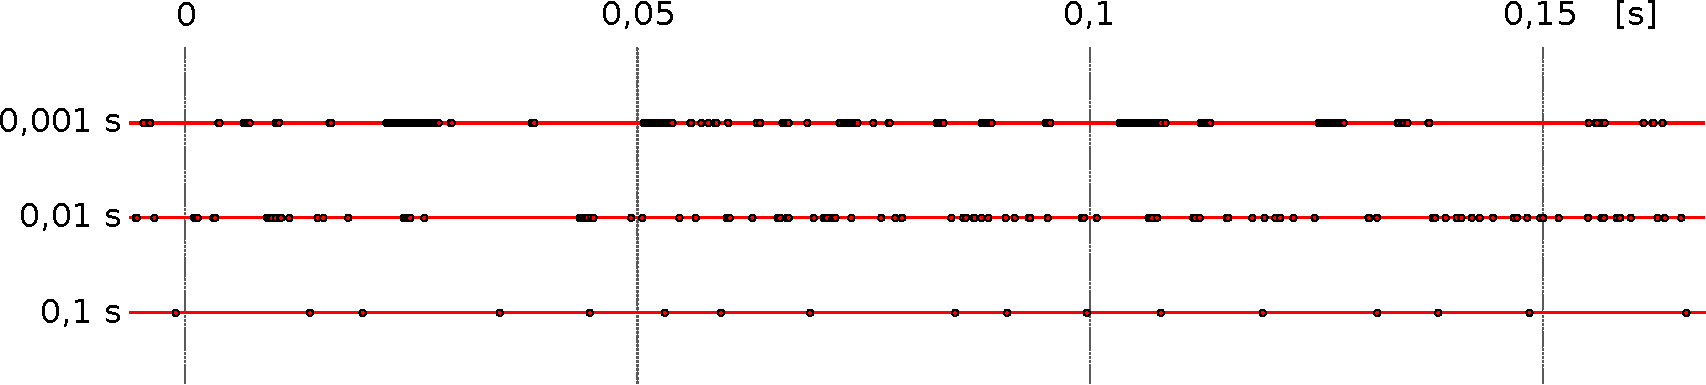
\includegraphics[width=\textwidth]{graphics/gramofon.pdf}
	\caption{Czas odbioru pakietu, wysyłanego przez program działający z jednym z trzech okresów.}
	\end{figure}
	
	Działa to tak samo, jakby każdą wiadomość wysyłać z losowym opóźnieniem.
	Gdy nadań jest za dużo (górny wykres), system zaczyna je buforować, a co za tym idzie, nadaje je w grupach o losowej wielkości.
	Pakiet po nadaniu przechodzi przez wiele procesów, każdy może nadawać losowe opóźnienie dla wiadomości.
	System operacyjny pod dużym obciążeniem przez inne procesy będzie opóźniał i buforował wiadomości o niższych częstotliwościach.
	
	Aby rozwiązać ten problem, należałoby uruchomić całe środowisko ROSa na systemie operacyjnym czasu rzeczywistego,
	również z tym pakietem.
	
\section{Podłoże o zmiennym współczynniku tarcia}
	Robi się to wewnętrznie w identyczny sposób, jak w przypadku kół platformy, co zostało opisane w sekcji \ref{sec:friction}.
	
	W tym przypadku jednak powinno się ustawić identyczne wektory tarć $f_0$ i $f_1$, aby podłoże symulowało równe tarcie we wszystkich kierunkach.
	Tak samo, jak w przypadku modelu platformy dynamicznej, program nadający podłożu odpowiednie wektory tarcia przyjmuje asynchroniczne wywołanie 
	typu \texttt{omnivelma\_msgs/SetFriction}, zawierające dwie wartości zmiennoprzecinkowe.
	
	
\section{Algorytm usuwania szumu z danych jednostki inercyjnej}
	Odczytuje nazwę nadajnika i odbiornika wiadomości typu \texttt{sensor\_msgs/Imu}, oraz wielkość bufora,
	Używany jest w przeprowadzeniu testów w sekcji \ref{sec:test_imu}.
	Program działa na zasadzie listy, do którego początku dodaje dane z nowych wiadomości, a z końca usuwa dane ze starych.
	Z każdą otrzymaną wiadomością, liczy średnią z aktualnie przechowywanych wyników.
	
\section{Obserwator symulacji}
	Wtyczka symulatora Gazebo, oblicza i zwraca ciąg danych, reprezentujący 
	odległość i kąt pomiędzy modelem dynamicznym, a kinematycznym, wiadomość \texttt{omnivelma\_msgs/Relative}.
	Te dane pozwalają sprawdzić, na ile symulacja fizyczna opóźnia się względem matematycznego modelu.
	
	Ten program nie może być zaimplementowany jako zewnętrzny pakiet, gdyż wiadomości zawierające pozycje platform będą przychodzić asynchronicznie.
	Nie da się w takim przypadku obliczyć dokładnych odległości pomiędzy platformami w danej chwili. 
	Wprowadzałoby to także spore opóźnienie, gdyż program musiałby czekać na odbiór obu wiadomości, dodatkowo zachowując pewność że oba pochodzą z tego samego kroku symulacji.
	
	Z punktu widzenia symulacji, program nie steruje modelem, a całą symulacją. Jest umieszczany w elemencie \texttt{word} pliku opisującego symulację,
	a nie w elemencie \texttt{model}. W związku z tym nie posiada symulowanej pozycji i prędkości. 
	Jednakże, bazując na nazwie, może sterować dowolnym obiektem w przestrzeni symulacji.
	W związku z tym, na diagramie \ref{uml:comparison}, został przedstawiony jako niezależny element uczestniczący w symulacji.
	
\section{Model kinematyki odwrotnej}
	Zaimplementowany jest w standardowy sposób typu akcja-reakcja.
	Odbiera wiadomość z zadanymi prędkościami liniowymi i rotacją, a zwraca wiadomość z prędkościami kół.
	
\section{Scena z symulacją}
	Plik typu \texttt{world} jest plikiem SDF, podobnym do tych, które służą do określenia wewnętrznej budowy robotów.
	Posiada listę elementów \texttt{import} ze ścieżkami modeli, a także nazwy programów działających bez modelu, jak obserwator symulacji, opisany w sekcji \ref{sec:ocznica}.

\section{Rozdzielacz wiadomości}
	Ten program wykonywalny pobiera i generuje wiadomości typu \texttt{omnivelma\_msgs/Vels}, zawierające prędkości kół.
	Pozwala to na sterowanie kilkoma robotami o identycznym interfejsie ze wspólnego źródła.
	W szczególności przydaje się to przy rozdzielaniu wartości prędkości kół dla modelu platformy dynamicznej i kinematycznej.

\section{Prosty program sterujący}
	Działanie programu oparte jest na zachowaniu akcja-reakcja.
	Dane z czujników laserowych dzielone są, w zależności od kąta pomiaru, na cztery ćwiartki lokalnego układu współrzędnych.
	Rozpatrywane są tylko te ćwiartki, w których kierunku porusza się platforma.
	Jeśli pomiar wypadnie wystarczająco blisko platformy, kierunek jest obracany w odwrotnym do tej ćwiartki kierunku.
	
	Na przykład, jeśli platforma porusza się w prawo i wykryje obiekt w trzeciej ćwiartce (czyli po prawej stronie względem aktualnego kierunku poruszania się),
	to zacznie poruszać się prosto, aby uniknąć przeszkody.
	
	Taki program gwarantuje omijanie przeszkód, aby platforma nie zderzyła się z jakimś obiektem.
